\section{Publications}
\label{sec:pubs}

This section gives pointers to recent publications about the three CV tasks:  {\em visual saliency, object/scene identification and image classification} as well as some work on frameworks for {\em large-scale} CV systems.

\subsection{Saliency}

The research question is how can the CV system determine automatically the most visually {\em salient} region(s) in an image? Saliency refers to distinctiveness (standing out), catching the focus of attention, characteristic. Usually a salient object of interest is sought to be separated from the background. Automatic measures of saliency are based on measurable properties of the object,
like texture, color, location and also simulating human visual attention.

A bottom-up visual saliency model, the {\em Graph-Based Visual Saliency (GBVS)} is proposed in \cite{Harel07graph-basedvisual}. The model is simple and biologically inspired based on activation maps of certain feature channels followed by normalization and combination with other maps. The GBVS outperforms by far the classical algorithms of Itti \& Koch \cite{Itti_Koch01nrn}. For the software, see  section \fullref{subsec:salmap}.

The salient object detection is formulated as image segmentation problem in \cite{LiuCVPR2007}. The object is separated from the background on the basis of several features including multi-scale contrast, center-surround histogram and color spatial distribution for the object description on several levels- locally, regionally and globally. The multi-scale contrast is the local feature, the center-surround histogram is the regional feature and the color spatial histogram- the global. These features are illustrated on Figure \ref{fig:sal_feat_liu07}.
\begin{figure}[H]
\begin{center}
\includegraphics[width=0.75\textwidth]{fig/SalientFeatures_Liu2007}
\end{center}
\caption{Examples of salient features. From left to right: input image, multi-scale contrast, center-surround histogram, color spatial distribution and binary salient mask by CRF.}
\label{fig:sal_feat_liu07}
\end{figure}
A Conditional Random Field (CRF) is trained on these features. 
For the purposes of this research the authors have compiled a large-scale database, MSRA (\cite{msra_db}), presented in section \fullref{subsec:msra}. The database is publicly available, while the software is not. The proposed methods, compared to two other algorithms ``FG" (fuzzy growing) and ``SM" (salient model as computed by the SalientToolbox, described in section \fullref{subsec:saltool}), tend to produce smaller and more focused bounding boxes.

Butko et al. in \cite{ButkoZCM08} propose fast approximation to a Bayesian model of visual saliency. The algorithm have been designed for efficiency in social robotics situations with the goal to orient a cameras as quickly as possible towards human faces. For the available software, see section \fullref{soft:fastsal:subsec}.

In \cite{LCAV-CONF-2009-012} the authors perform a frequency-domain analysis on five state-of-the-art saliency methods, and compared the spatial frequency
content retained from the original image, which is then used in the computation of the saliency maps. This analysis illustrated that the deficiencies of these techniques
arise from the use of an inappropriate range of spatial frequencies. Based on this analysis, they presented a frequency-tuned
approach of computing saliency in images using low level features of color and luminance. The resulting saliency maps are better suited to salient object segmentation, with higher precision and better recall than the analyzed state-of-the-art techniques. For the available software, see section \fullref{subsec:freqsal}.

In \cite{YanCVPR2013} the authors address a fundamental problem in saliency detection, namely, the small-scale background structures, which affect the detection. This problem occurs often in natural images. They propose a hierarchical framework that infers importance values from image layers with different scales. The approach is summarized in Figure \ref{fig:hier_yan13}.

\begin{figure}[H]
\begin{center}
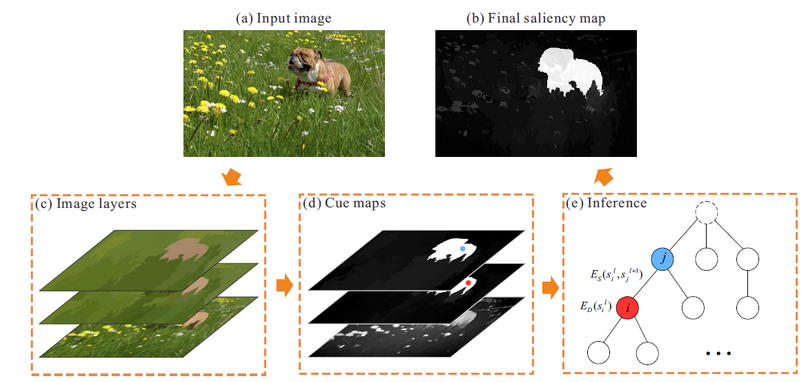
\includegraphics[width=0.9\textwidth]{fig/Hierarchy_Yan13}
\end{center}
\caption{An overview of the hierarchical framework. Three image layers are extracted from the input, and then  saliency cues from each of these layers are computed. They are finally fed into a hierarchical model to get the final results.}
\label{fig:hier_yan13}
\end{figure}

For the purpose of their research the authors made a new database available to the community, the Complex Scene Saliency Dataset (CSSD) and the Extended CSSD (ECSSD), described in Section \fullref{subsec:cssd}. The executable of their software is also available from the project link (\cite{ecssd_db}), but not the source code. The authors report better performance of their method compared to $11$ other state-of-the-art methods.

Recently, a method for statistical textural distinctiveness for detecting saliency in natural images have been proposed \cite{texstatdist2013}. Textural representations are extracted and a sparse models learned. Next, a weighted graphical model is constructed and used to distinguish between all texture atom pairs.

\subsection{Salient regions}

For the {\em object/scene identification} task, the main question is whether two images taken at different times or under different conditions depict the same object/scene. One approach is to compare sets of local characteristic features, extracted reliably and independently from the two images.

Detecting automatically {\em salient}, e.g.  interesting, distinct, characteristic and repeatably find-able regions from an image is a major research topic in the area of image {\em feature extraction}. The salient regions are one type of features, which can offer useful representation of images, along with interest points, edges, ridges etc. Usually the first step is automatically extracting salient regions using an salient/interest region {\em detector} followed by describing each region/patch using a region {\em descriptor}. This is illustrated in Figure \ref{fig:keydescr}.

\begin{figure}[H]
\begin{center}
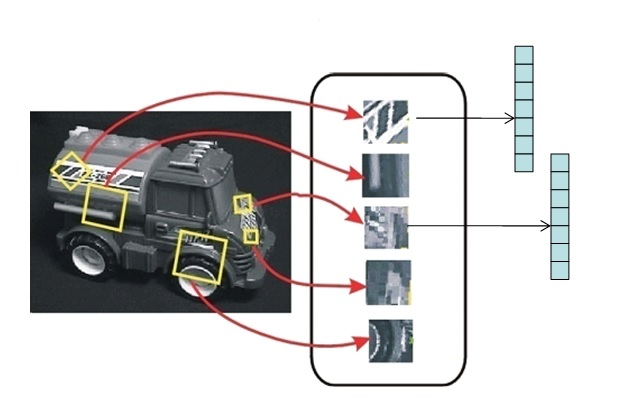
\includegraphics[width=0.5\textwidth]{fig/KeypointsDescriptors}
\end{center}
\caption{Extracting descriptors from detected keypoints/regions.}
\label{fig:keydescr}
\end{figure}

As a final step, two sets of region descriptors are compared and {\em matched} in order to establish correspondences between the images.

One very important and desired property of such region detection is {\em affine covariance} (often referred to as {\em affine invariance}).  The affine covariance refers to the requirement that these regions should correspond to the same pre-image for different viewpoints and geometric transformations. This concept is shown on Figure \ref{fig:affreg}. The figure illustrates that an affine salient regions detector has automatically and independently detected the same pre-image regions on both images. Some detectors provide arbitrarily shaped regions, others detect elliptical regions. For the purpose of comparison, the (equivalent) elliptical regions are usually used for display.
\begin{figure}[H]
\begin{center}
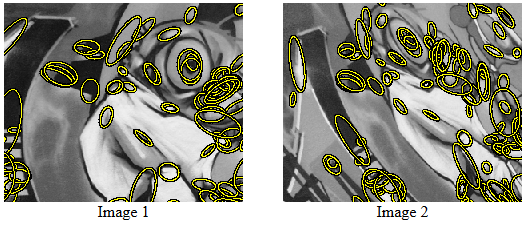
\includegraphics[width=0.6\textwidth]{fig/AffineRegions}
\end{center}
\caption{Example of affine regions detection. Image2 is affinely transformed version of Image1.}
\label{fig:affreg}
\end{figure}

\subsubsection{Detectors}
A decade ago, a seminal paper by the Visual Geometry Group in Oxford, compared the existing affine-covariant region detectors in \cite{Mikolajczyk:2005}. A clear conclusion of this comparative study is the the  {\em  Maximally Stable Extremal Regions (MSER)} detector (\cite{Matas2002BMVC}) is the winner in many of the test scenarios and since then, the MSER detector has become a de-facto standard in the field (for example is now an integral part of the MATLAB Computer Vision System Toolbox). For common implementations of MSER, the reader is referred to section \fullref{soft:salregdet:subsec}.

After this comparative study, several researchers have proposed improvements to the MSER detector, though none of them increased the performance drastically. 
An MSER color extension is proposed in \cite{Forssen07}. The author calls his detector {\em Maximally Stable Color Region (MSCR)}. In comparison to the original MSER detector, the simple color MSER extension (MSER3) and a color blob detector, the MSCR performs the best in most cases on the well-known Visual Geometry Group in Oxford test image sets with known homographies (\cite{vgg_soft_data}). 

The MSER detector has been also extended in 3D to {\em Maximally Stable Volumes (MSVs)} in \cite{DonoserB06}. The MSVs have been used to successfully segment 3D medical images and paper fiber networks.

A {\em Structure-Guided Salient Region detector (SGSR)} is introduced in \cite{Fan08}. It is based on entropy-based saliency theory and shows competitive performance.

Another enhancement of MSER with the Canny edge detector is introduced in \cite{Wang14}. The dilation operator is used on the detected edges to remove ambiguous edges, which makes the interest regions more representative. The improved MSER shows better performance than the original MSER in image classification in the bag of words framework, though original comparison of repeatably (\cite{Mikolajczyk:2005}) is not presented. 

In the context of humpback whale identification, Ranguelova et al. have proposed {\em Morphology based Stable Salient Regions (MSSR)} detector \cite{RangMSSR06, RangHumpb06} . MSSR is not better than MSER on repeatably, but produces less number of regions (which is important in the matching step) and better represents human salient perception. Within the eStep, NLeSC's technology platform, some research is ongoing to improve MSSR.

Links to the implementations of the detectors are given in section \fullref{soft:salregdet:subsec}.

\subsubsection{Descriptors}
Another important performance evaluation paper from the Oxford Vision group has compared the salient region descriptors \cite{MS05}. The conclusion of the performance evaluation was that the {\em Gradient Location-Orientation Histogram (GLOH)} detector was performing best (recall and precision) followed closely by the {\em Scale Invariant Feature Transform (SIFT)} descriptor \cite{Lowe:2004}. The SIFT descriptor has been the most popular and widely used descriptor in CV for over a decade. 

The idea behind SIFT Transform is finding the extrema rom all possible scales and image locations (scale space). From these potential interest points only the most stable points are selected. One or more orientations are assigned to a point based on the local gradient directions, while invariance to transformations is achieved by computing these orientations from all possible transformed versions of the data.  This histogram of (usually $128$) orientations are the keypoint descriptor (Figure \ref{fig:sift}). The SIFT descriptor is example of descriptors based on Histogram of Gradients (HoG). For applying SIFT descriptor on salient regions, only the descriptor steps are performed. 

\begin{figure}[H]
\begin{center}
\includegraphics[width=0.6\textwidth]{fig/SIFT}
\end{center}
\caption{SIFT descriptor steps. From left to right: keypoint detection; image gradients; descriptor.}
\label{fig:sift}
\end{figure}

An algorithm for GPU-based video tracking and matching has been published at \cite{Sinha06gpu-basedvideo}. There are many variants of the SIFT descriptor, all based on floating point arithmetic, for example, SURF\cite{Bay:2008:SURF} and also GLOH \cite{MS05}, designed to improve distinctiveness.  

Other alternatives to SIFT are {\em FAST} \cite{Rosten:2006}, which compares pixels on a ring centered at a feature point. {\em  ORB} \cite{Rublee:2011} extends FAST by computing orientations based on the intensity centroid moment. Rotation invariance is also achieved with the MRRID and MROGH descriptors, \cite{journals:pami:FanWH12} by pooling local features based on their intensity orders. In the same group is the {\em Local Intensity Order Pattern (LIOP)} descriptor \cite{ZhenhuaWang:2011:LIO}. 

Another important class of descriptors which offer computationally more tractable solution to region/patch description, are the {\em binary descriptors}. Unlike SIFT or SURF and the expensive computation of gradients, a set of simple binary tests are used with the Hamming distance. Examples of such descriptors are {\em Binary Robust Independent Elementary Features (BRIEF)}\cite{Calonder:2010}, {\em Binary Robust Invariant Keypoints (BRISK)} \cite{Leutenegger:2011}, etc. A binary descriptor is composed of three parts:
\begin{enumerate}
\item{\bf Sampling pattern}. Where to sample points in the region around the interest point.
\item{\bf Orientation compensation}. Measure the orientation of the keypoint and rotate it to compensate for rotation.
\item{\bf Sampling pairs}. Which pairs to compare when building the final descriptor.
\end{enumerate}
For all possible sampling pairs a binary test is performed. For each pair $(p_1, p_2)$, if the intensity at point $p_1$ is greater than the intensity at point $p_2$, the descriptor value for that pair is $1$, otherwise $0$ (Figure \ref{fig:bindescr}). A very good tutorial on binary descriptors can be found \href{https://gilscvblog.wordpress.com/?s=descriptors}{\underline{online}}. 

\begin{figure}[H]
\begin{center}
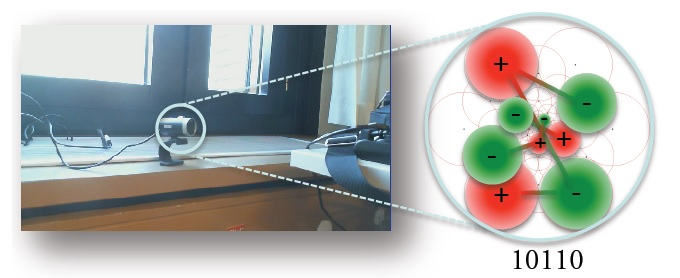
\includegraphics[width=0.5\textwidth]{fig/BinDescr}
\end{center}
\caption{Binary descriptor.}
\label{fig:bindescr}
\end{figure}

Another more recent performance paper compares their performance also in comparison to the established descriptors like SIFT or SURF \cite{conf:icpr:MiksikM12}. The main conclusions of the evaluation are:
\begin{enumerate}
\item{The real valued descriptors such as LIOP, MRRID and MROGH outperform SUFR and SIFT both in precision and recall, although with low efficiency.}
\item{The binary descriptors are very efficient for time-constrained applications with good matching accuracy}
\item{The binary descriptors are very fast with low memory requirements ($32$ bytes for BRIEF and ORB or $64$ bytes for BRISK). These provide comparable precision/recall to SIFT/SURF.}
\end{enumerate}

A very recent descriptor, {\em Binary Online Learned Descriptor (BOLD)}, \cite{Balntas_2015_CVPR} has been proposed. It combines the advantages of an efficient binary descriptor with the improved performance of learning-based descriptors. The binary tests are learned from the content of the patches themselves minimizing the intra-class distances leading to a more robust descriptor. BOLD has a good performance both in terms of accuracy as well as efficiency.

Links to the implementations of the detectors are given in section \fullref{soft:salregdescr:subsec}.
\subsubsection{Matching}
The extracted descriptors from the detected regions (as blobs or around keypoints) are usually compared via nearest neighborhood (NN) search. Much research is done for developing algorithms for faster matching. The most popular approaches are using kd-trees and hashing methods (see \cite{conf:icpr:MiksikM12} and the references within). For binary descriptors matching is performed efficiently using Hamming distance, {\em xor} and {\em population count}.


\subsection{Convolutional Neural Networks}

The current trend of research to solve the most challenging task in CV, object/scene classification, is deep learning. {\em Deep Machine Learning} has been declared the new frontier in artificial intelligence research in 2010, \cite{Arel:2010}. It has been inspired by the findings of neuroscience that the neocortex, which is associated with many cognitive abilities, does not explicitly pre-process sensory signals, but rather allows them to propagate through a complex hierarchy that, over time, learn to represent observations based on their regularities \cite{Lee1998,Lee03}. This  motivated the emergence of the deep machine learning, which focuses on computational models that exhibit similar characteristics. The main goal of deep learning is to train multi-layered (deep) hierarchical network on large set of observations to extract signals from this network to a relatively simple classification engine for the purpose of robust (invariant to a diverse range of transformations and distortions) pattern recognition.

The {\em Convolutional Neural Networks (CNN)} are a type of deep learning networks \cite{Bengio:2009}. CNNs are a family of multi-layer neural networks particularly designed for use on two-dimensional data, such as images and videos. In CNNs, small portions of the image (a local receptive field) are treated as inputs to the lowest layer of the hierarchical structure. Information generally propagates
through the different layers of the network whereby at each layer digital filtering is applied in order to obtain salient features of the data observed. The method provides a level of invariance to
shift, scale and rotation as the local receptive field allows the neuron (processing unit) access to low-level features such as oriented edges or corners. The filtering is a {\em convolution} with filter, followed by sub-sampling to further decrease the dimensionality and provides invariance to shifts (Figure \ref{fig:conv}).

\begin{figure}[H]
\begin{center}
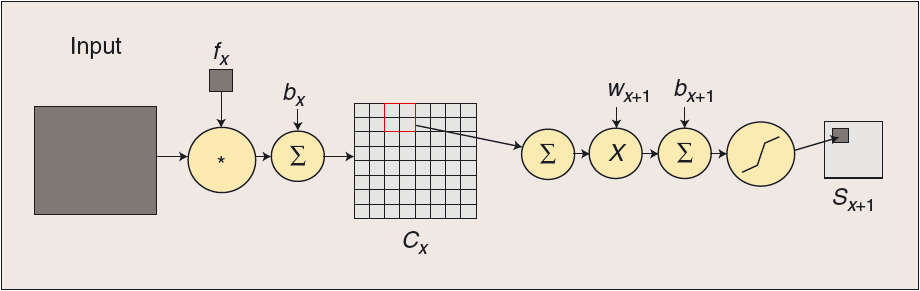
\includegraphics[width=0.65\textwidth]{fig/Conv}
\end{center}
\caption{The convolution and sub-sampling. Convolving an input (image for the first stage or feature map for later stages) with a trainable filter $f_x$ and adding a trainable bias $b_x$
to produce the convolution layer $C_x$. The sub-sampling is summing a neighborhood ($4$ pixels), weighting by scalar $w_{x+1}$, adding trainable bias $b_{x+1}$, and
passing through a sigmoid function to produce a twice smaller feature map $S_{x+1}$.}
\label{fig:conv}
\end{figure}

The convolution an sub-sampling can be performed arbitrary number of times. A conceptual example of CNNs is shown on Figure \ref{fig:cnn}. CNNs create their invariance to object translations by a {\em ``feature pooling ''} (the $S$ layers in Figure \ref{fig:cnn}). 

\begin{figure}[H]
\begin{center}
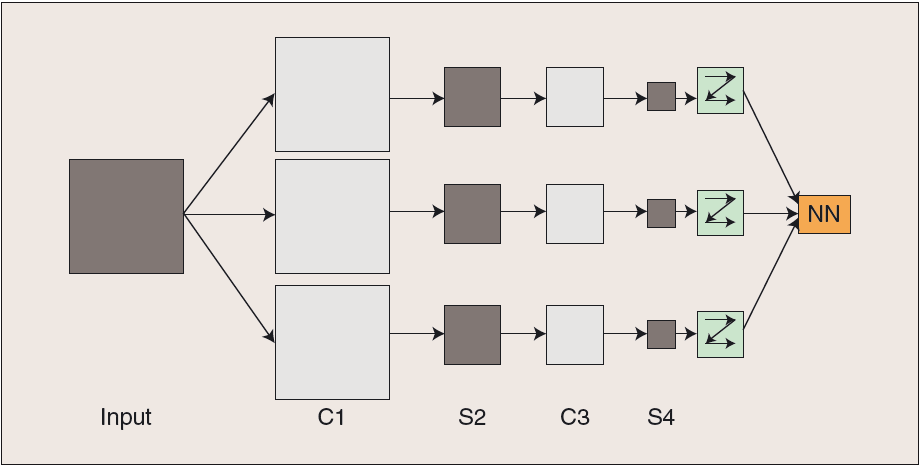
\includegraphics[width=0.65\textwidth]{fig/cnn}
\end{center}
\caption{Conceptual example of CNN. The input image is convolved with $3$ trainable filters and biases as in Figure \ref{fig:conv} to produce $3$ feature maps at the $C_1$
level. Each group of $4$ pixels in the feature maps are added, weighted, combined with a bias, and passed through a sigmoid function to produce the $3$ feature maps at $S_2$. These are again
filtered to produce the $C_3$ level. The hierarchy then produces $S_4$ in a manner analogous to $S_2$. Finally these pixel values are rasterized and presented as a single vector input to the “conventional” neural network at the output.}
\label{fig:cnn}
\end{figure}

The close relationship between the layers and spatial information in CNNs makes them well suited for image processing and understanding, and they generally perform well at autonomously extracting salient features from images. Since then, especially after the CNNs performed better than the hand-crafted features in the ImageNet challenge \cite{ILSVRC15}, a lots of research has been done in CNNs in CV. 
Here we mention only few key papers.For a starting point to the large amount of publications on the topic the reader is referred to the \href{http://deeplearning.net/reading-list/}{\underline{reading list}} of the DeepLearning.net. Also, all papers from the last $3$ years of the largest CV conference Computer Vision and Pattern Recognition (CVPR)  are available \href{http://www.cv-foundation.org/openaccess/menu.py}{\underline{online}}.

Despite the CNN success, to a large extend they are still 'black boxes' and researchers try to get deeper insight of the internal working of the network, namely to understand
the representations that are learned by the inner layers of these deep architectures. As scenes are composed of objects, the CNN for scene classification
automatically discovers meaningful objects detectors, representative of the learned categories. With object detectors emerging as a result of learning to
recognize scenes,\cite{ZhouKLOT14} demonstrates that the same network can perform both scene recognition and object localization in a single forward-pass (Figure \ref{fig:cnn_objdet}), without
 explicitly learning the notion of objects. 

\begin{figure}[H]
\begin{center}
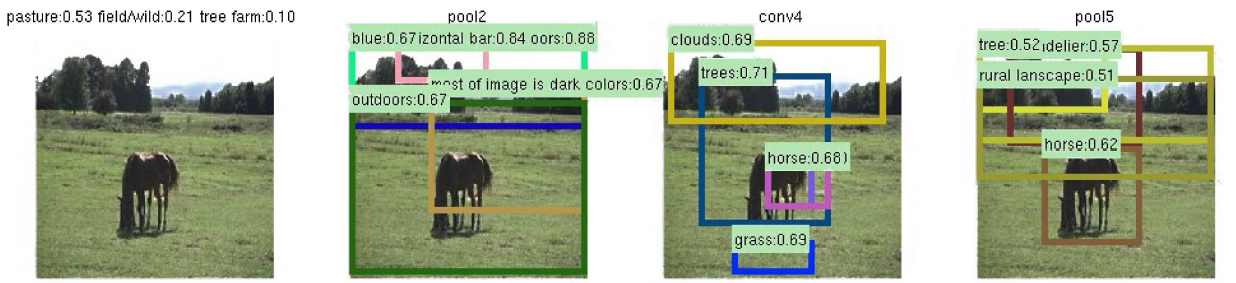
\includegraphics[width=0.75\textwidth]{fig/cnn_objdet}
\end{center}
\caption{Interpretation of a picture by different layers of the Places-CNN (\fullref{subsec:places}) using semantic tags given by humans. The first shows the final layer output of Places-CNN. The other three show
detection results along with the confidence based on the units’ activation and the semantic tags.}
\label{fig:cnn_objdet}
\end{figure}

Another approach for trying to understand the CNNs is by ``fooling'' them! Researchers have shown that  it is easy to produce images that are
completely unrecognizable to humans, but that CNNs believe to be recognizable objects with $99.99\%$ confidence (e.g. labeling with certainty that white noise
static is a lion). These are called  “fooling images” (Figure \ref{fig:cnn_fool}), \cite{NguyenYC14}. These results shed light on interesting differences
between human vision and current CNNs, and raise questions about the generality of CNN computer vision.

\begin{figure}[H]
\begin{center}
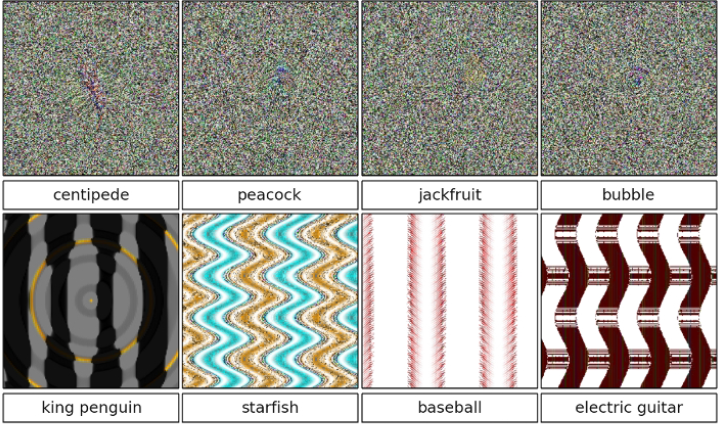
\includegraphics[width=0.65\textwidth]{fig/cnn_fool}
\end{center}
\caption{Evolved images that are unrecognizable to humans, but that CNN trained on ImageNet believe with
$99.6\%$ certainty to be a familiar object. This result highlights differences between how CNNs and humans recognize objects.
Images are either directly (top) or indirectly (bottom) encoded.}
\label{fig:cnn_fool}
\end{figure}

Another fundamental issue with the CNN is the need for many {\em labeled} observations for training. This could be a serious obstacle for the application of CNNs. Interesting trend are the {\em never ending learning systems}. For example, \href{http://www.neil-kb.com/}{\em \underline{NEIL}} {\em (Never Ending Image Learner)} is a computer program that runs $24$ hours per day and $7$ days per week to automatically extract visual knowledge from Internet data. For more details see \cite{Chen_2013_ICCV}. 

Recently, an interesting article which compares the matching of salient regions with CNNs with matching with SIFT descriptor have been published \cite{FischerDB14}. The authors have also recorded a new larger dataset, compared to the only $48$ images in the comparative study paper, covering larger class of image transformations with more images (see \fullref{sec:salregdb}). The goal of the paper is to study the regions/patches descriptors, not to evaluate detectors. For the detection step, the standard MSER detector have been used. The paper concludes that the CNN trained features are consistently better than the SIFT descriptor, for the price of a higher computational cost.

Software packages supporting CNNs are given in Section \fullref{soft:DL:subsec}.

\subsection{Large Scale CV Systems}
One of the manifestations of the Big Data era is the proliferation of massive visual data. The key challenges in extracting a value from these data are:
\begin{itemize}
\item{ {\bf Scalability.} This is the key challenge in the world of Big Data. Lack of infrastructural support leaves researcher repeatedly facing the same difficulties when developing and porting  distributed CV algorithms.}
\item{\bf Provably Correct Parallel/Distributed Implementations.} Designing and implementing
efficient and correct parallel computer vision algorithms is extremely challenging. Some tasks like extracting statistics from image collections are embarrassingly parallel, i.e. can be parallelized simply by distributing
the images to different machines. Unfortunately, most tasks in CV and
machine learning such as training a face detector are not embarrassingly parallel
(there are data and computational dependencies between images and various
steps in the algorithm).
\item{\bf Reusability.} Computer vision researchers have developed vision algorithms
that solve specific tasks but software developers building end-to-end system
find it extremely difficult to integrate these algorithms into the system due to
different software stacks, dependencies and different data format.
\end{itemize}
Researchers are looking more and more at these challenges.

\subsubsection{MapReduce}

{\em MapReduce} is a programming model and its implementation for processing large datasets, introduced by Google, \cite{Dean:2008}. The user specifies the computations in terms of {\em map} and {\em reduce} functions, and the system automatically parallelizes the computation across large clusters of machines at run-time. Generally CV algorithms are applied on one or more images, consisting of pixels with some set of potentially varying parameters. Parallelism can be exploited on any of these levels, across parameters the task is embarrassingly parallel (i.e.independant) and on image or pixel level,the parallelization depends on whether the algorithm operates independently (e.g. SIFT, face detection).

For example \cite{White:2010} addresses a web-scale multimedia mining task using MapReduce. The paper describes the low level implementation of several computer vision algorithms relevant for mining applications: classifier training, sliding windows, clustering, bag-of-features, background subtraction and image registration.  The paper gives guidelines and algorithms of how the mappers and reducers can be implemented for some CV tasks. For example, for classifier training, the mapper performs the feature computation in parallel, the features are collected for the reducer where the classifier training is performed. 

A further development in that direction is the {\em Hadoop Image Processing Interface (HIPI)} library \cite{hipi_soft}. The undergraduate thesis of C. Sweeney is the publication about HIPI \cite{hipi_pub}. The goal of HIPI is to provide a simple and clean interface for high-throughput distributed image processing on the MapReduce platform. Figure \ref{fig:hipi} illustrates a typical MapReduce/HIPI workflow.

\begin{figure}[H]
\begin{center}
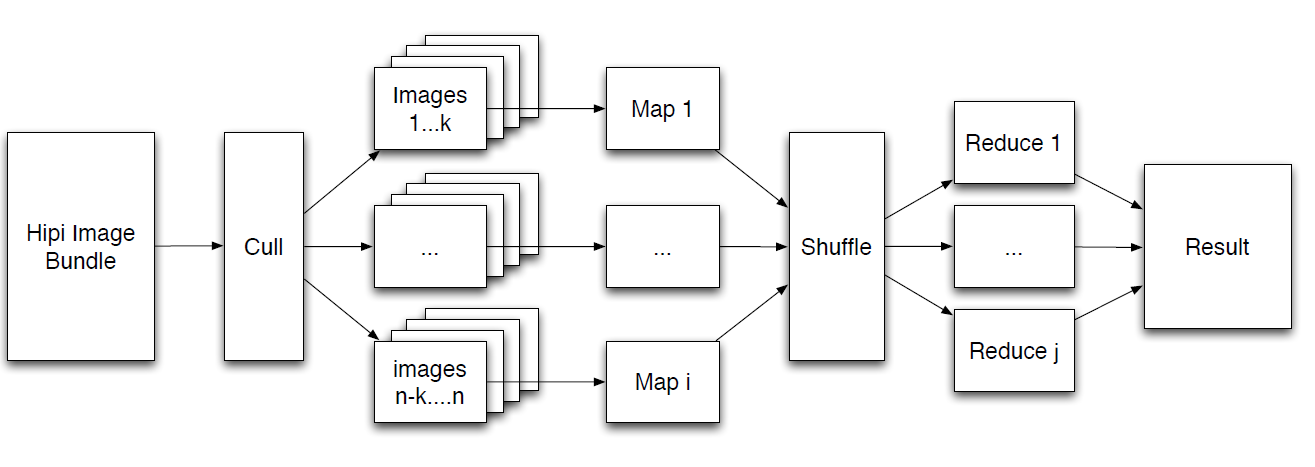
\includegraphics[width=0.8\textwidth]{fig/HIPI}
\end{center}
\caption{A typical MapReduce pipeline using HIPI with $n$ images, $i$ map nodes and $j$ reduce nodes.}
\label{fig:hipi}
\end{figure}
HIPI is designed to abstract Hadoop's functionality into an image-centric system and to serve as a tool for efficient use of Hadoops MapReduce for image processing and computer vision.
For the MapReduce/HIPI software, see Section \fullref{subsubsec:MapReduce}.

\subsubsection{Cognitive Computer Vision Systems}
Apart from traditional research of CV algorithms, in the last decades much research has been done into integrating such algorithms into larger systems. For example, {\em cognitive computer vision (CVS) systems} does not only involve CV, but also {\em machine learning} and reasoning to extend priory knowledge or verify the consistency of results. An overview paper studies the requirements and developments for large scale CVS, \cite{WredeBSPV04}. The existing systems have been evaluated along {\em functional , non-functional and additional requirements} illustrated on Figure \ref{fig:cvseval}.

The study groups the frameworks in $4$ major classes based on the evaluation.  

\begin{enumerate}
\item{{\em Visual Image Processing Environments}, e.g.ImaLab (see Figure \ref{fig:cvseval}) provides facilities to quickly develop pipelines and allows rapid prototyping, easy GUI. They lack support for distributed architectures.}
\item{{\em Middleware approaches}, e.g. COBRA implementation TAO. Very generic and powerful, but complicated use. Also do not support specific CV domain requirements.}
\item{{\em Robotics domain}, e.g.SmartSoft or OROCOS. Satisfy many CV requirements, including distribution and transparency. However, their integration is largely coupled with the robot control components.}
\item{{\em CVS Frameworks}, {\bf XCF} \cite{Wrede2004-AXB} focuses on data management
facilities, distribution and rapid prototyping, {\bf zwork} \cite{ponweiser2003reusable} mainly deals with the programmatic coordination and
dynamic reconfiguration in the control aspect of CVS.}
\end{enumerate}

\begin{figure}[H]
\begin{center}
\includegraphics[width=0.45\textwidth]{fig/CVSEval}
\end{center}
\caption{Graphical evaluation scheme for CVS (ImaLab). Each assessment category has $5$ step scale: '--'- impossible, '-'- difficult, 'o'- neutral, '+'- supported and '++'- automatic.}
\label{fig:cvseval}
\end{figure}

Therefore, the system engineers will have to carefully identify their needs and project requirements and correspondingly decide for a most suitable framework.

\subsubsection{CloudCV}
A very recent development, which tackles the large-scale CV challenges, is the \href{http://cloudcv.org/}{\underline{CloudCV}}, \cite{AgrawalMGCBMOB15}. The goal is to democratize computer vision, i.e. make the state-of-the-art distributed CV algorithms also available to non-experts (i.e. people who are not CV researchers or Big Data experts). Therefore, the platform aims at three different audiences: computer vision researcher, scientists which are not CV experts and non-scientists. 

CloudCV consists of a group of virtual machines running on Amazon
Web Services capable of running large number of tasks in a distributed and parallel
setting. Popular datasets are already cached on these servers to facilitate researchers
trying to run popular computer vision algorithms on these datasets. For custom datasets the users
can access these services through a web interface for uploading smaller sets, or use Python and Matlab APIs for larger datasets. An overview of the system is shown on Figure \ref{fig:cloudcv}.

\begin{figure}[H]
\begin{center}
\includegraphics[width=0.7\textwidth]{fig/CloudCV}
\end{center}
\caption{Overview of CloudCV.}
\label{fig:cloudcv}
\end{figure}

The paper presents the back-end infrastructure (web servers,distributed processing and job schedulers), the used deep learning framework and the front-end platforms (web interface, Python and MATLAB APIs). It also presents in detail the CloudCV functionalities, namely classification, feature extraction, finding VIP in group images, gigapixel image stitching. A very concrete future plan is to integrate the {\em Deep Learning GPU Training System} \href{https://developer.nvidia.com/digits}{\underline{\em (DIGITS)}}, \cite{digits_soft} with CloudCV. 